\documentclass[twoside]{book}

% Packages required by doxygen
\usepackage{fixltx2e}
\usepackage{calc}
\usepackage{doxygen}
\usepackage[export]{adjustbox} % also loads graphicx
\usepackage{graphicx}
\usepackage[utf8]{inputenc}
\usepackage{makeidx}
\usepackage{multicol}
\usepackage{multirow}
\PassOptionsToPackage{warn}{textcomp}
\usepackage{textcomp}
\usepackage[nointegrals]{wasysym}
\usepackage[table]{xcolor}

% Font selection
\usepackage[T1]{fontenc}
\usepackage[scaled=.90]{helvet}
\usepackage{courier}
\usepackage{amssymb}
\usepackage{sectsty}
\renewcommand{\familydefault}{\sfdefault}
\allsectionsfont{%
  \fontseries{bc}\selectfont%
  \color{darkgray}%
}
\renewcommand{\DoxyLabelFont}{%
  \fontseries{bc}\selectfont%
  \color{darkgray}%
}
\newcommand{\+}{\discretionary{\mbox{\scriptsize$\hookleftarrow$}}{}{}}

% Page & text layout
\usepackage{geometry}
\geometry{%
  a4paper,%
  top=2.5cm,%
  bottom=2.5cm,%
  left=2.5cm,%
  right=2.5cm%
}
\tolerance=750
\hfuzz=15pt
\hbadness=750
\setlength{\emergencystretch}{15pt}
\setlength{\parindent}{0cm}
\setlength{\parskip}{0.2cm}
\makeatletter
\renewcommand{\paragraph}{%
  \@startsection{paragraph}{4}{0ex}{-1.0ex}{1.0ex}{%
    \normalfont\normalsize\bfseries\SS@parafont%
  }%
}
\renewcommand{\subparagraph}{%
  \@startsection{subparagraph}{5}{0ex}{-1.0ex}{1.0ex}{%
    \normalfont\normalsize\bfseries\SS@subparafont%
  }%
}
\makeatother

% Headers & footers
\usepackage{fancyhdr}
\pagestyle{fancyplain}
\fancyhead[LE]{\fancyplain{}{\bfseries\thepage}}
\fancyhead[CE]{\fancyplain{}{}}
\fancyhead[RE]{\fancyplain{}{\bfseries\leftmark}}
\fancyhead[LO]{\fancyplain{}{\bfseries\rightmark}}
\fancyhead[CO]{\fancyplain{}{}}
\fancyhead[RO]{\fancyplain{}{\bfseries\thepage}}
\fancyfoot[LE]{\fancyplain{}{}}
\fancyfoot[CE]{\fancyplain{}{}}
\fancyfoot[RE]{\fancyplain{}{\bfseries\scriptsize Generated on Sat Sep 12 2015 15\+:54\+:41 for Ser321 C++ Media\+Client\+Gui by Doxygen }}
\fancyfoot[LO]{\fancyplain{}{\bfseries\scriptsize Generated on Sat Sep 12 2015 15\+:54\+:41 for Ser321 C++ Media\+Client\+Gui by Doxygen }}
\fancyfoot[CO]{\fancyplain{}{}}
\fancyfoot[RO]{\fancyplain{}{}}
\renewcommand{\footrulewidth}{0.4pt}
\renewcommand{\chaptermark}[1]{%
  \markboth{#1}{}%
}
\renewcommand{\sectionmark}[1]{%
  \markright{\thesection\ #1}%
}

% Indices & bibliography
\usepackage{natbib}
\usepackage[titles]{tocloft}
\setcounter{tocdepth}{3}
\setcounter{secnumdepth}{5}
\makeindex

% Hyperlinks (required, but should be loaded last)
\usepackage{ifpdf}
\ifpdf
  \usepackage[pdftex,pagebackref=true]{hyperref}
\else
  \usepackage[ps2pdf,pagebackref=true]{hyperref}
\fi
\hypersetup{%
  colorlinks=true,%
  linkcolor=blue,%
  citecolor=blue,%
  unicode%
}

% Custom commands
\newcommand{\clearemptydoublepage}{%
  \newpage{\pagestyle{empty}\cleardoublepage}%
}


%===== C O N T E N T S =====

\begin{document}

% Titlepage & ToC
\hypersetup{pageanchor=false,
             bookmarks=true,
             bookmarksnumbered=true,
             pdfencoding=unicode
            }
\pagenumbering{roman}
\begin{titlepage}
\vspace*{7cm}
\begin{center}%
{\Large Ser321 C++ Media\+Client\+Gui }\\
\vspace*{1cm}
{\large Generated by Doxygen 1.8.9.1}\\
\vspace*{0.5cm}
{\small Sat Sep 12 2015 15:54:41}\\
\end{center}
\end{titlepage}
\clearemptydoublepage
\tableofcontents
\clearemptydoublepage
\pagenumbering{arabic}
\hypersetup{pageanchor=true}

%--- Begin generated contents ---
\chapter{Hierarchical Index}
\section{Class Hierarchy}
This inheritance list is sorted roughly, but not completely, alphabetically\+:\begin{DoxyCompactList}
\item Fl\+\_\+\+Window\begin{DoxyCompactList}
\item \contentsline{section}{Media\+Client\+Gui}{\pageref{class_media_client_gui}}{}
\end{DoxyCompactList}
\end{DoxyCompactList}

\chapter{Class Index}
\section{Class List}
Here are the classes, structs, unions and interfaces with brief descriptions\+:\begin{DoxyCompactList}
\item\contentsline{section}{\hyperlink{class_media_client_gui}{Media\+Client\+Gui} \\*Copyright (c) 2015 Tim Lindquist, Software Engineering, Arizona State University at the Polytechnic campus }{\pageref{class_media_client_gui}}{}
\end{DoxyCompactList}

\chapter{File Index}
\section{File List}
Here is a list of all documented files with brief descriptions\+:\begin{DoxyCompactList}
\item\contentsline{section}{src/cpp/\hyperlink{_media_client_gui_8cpp}{Media\+Client\+Gui.\+cpp} }{\pageref{_media_client_gui_8cpp}}{}
\end{DoxyCompactList}

\chapter{Class Documentation}
\hypertarget{class_media_client_gui}{}\section{Media\+Client\+Gui Class Reference}
\label{class_media_client_gui}\index{Media\+Client\+Gui@{Media\+Client\+Gui}}


Copyright (c) 2015 Tim Lindquist, Software Engineering, Arizona State University at the Polytechnic campus.  


Inheritance diagram for Media\+Client\+Gui\+:\begin{figure}[H]
\begin{center}
\leavevmode
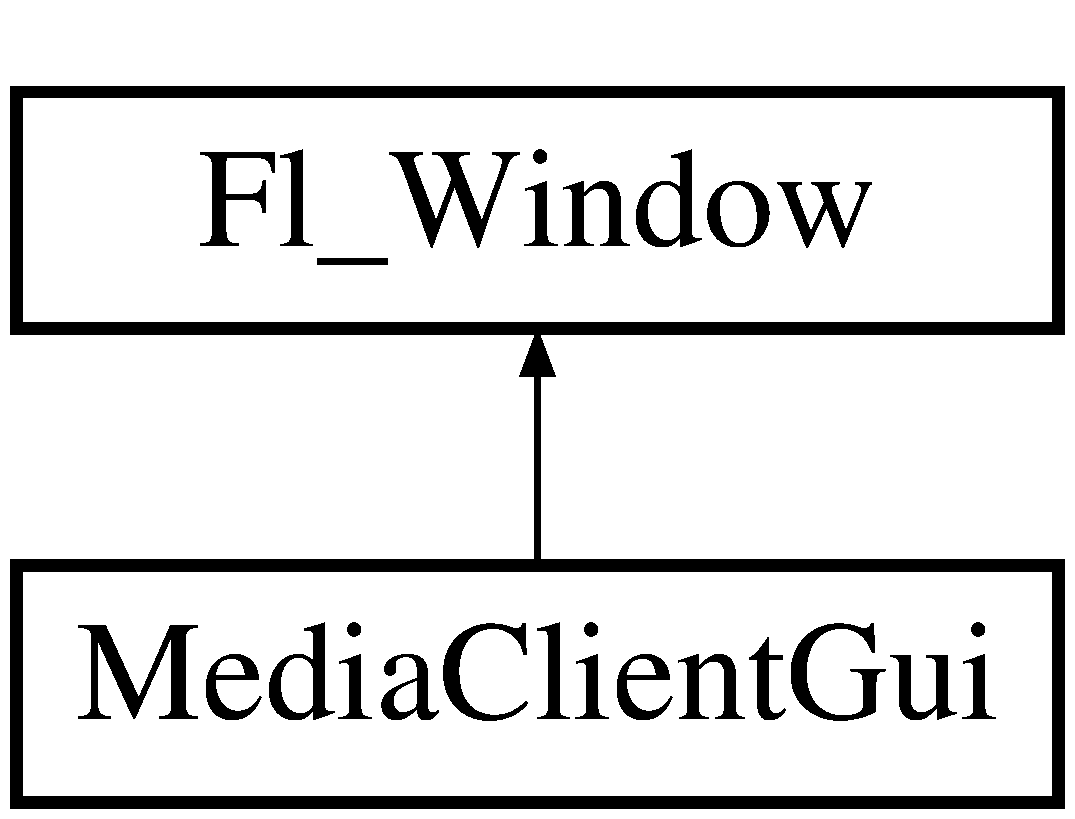
\includegraphics[height=2.000000cm]{class_media_client_gui}
\end{center}
\end{figure}
\subsection*{Public Member Functions}
\begin{DoxyCompactItemize}
\item 
\hyperlink{class_media_client_gui_a73eeabbba329bd1b7f558d65e0c3eab3}{Media\+Client\+Gui} (const char $\ast$name=\char`\"{}Ser321\char`\"{})
\begin{DoxyCompactList}\small\item\em A Constructor for \hyperlink{class_media_client_gui}{Media\+Client\+Gui} Constructor taking a c-\/string argument, which is used as a window label for the client application. \end{DoxyCompactList}\end{DoxyCompactItemize}
\subsection*{Protected Attributes}
\begin{DoxyCompactItemize}
\item 
Fl\+\_\+\+Tree $\ast$ \hyperlink{class_media_client_gui_a271cf7771f269da55fbe873f17238ab2}{tree}
\begin{DoxyCompactList}\small\item\em tree is the Fl\+\_\+\+Tree object that occupies the left side of the window. \end{DoxyCompactList}\item 
Fl\+\_\+\+Input $\ast$ \hyperlink{class_media_client_gui_a3e4fe22653dbf41f11c14f5a572e79c8}{title\+Input}
\begin{DoxyCompactList}\small\item\em title\+Input is the Fl\+\_\+\+Input object labelled Title. \end{DoxyCompactList}\item 
Fl\+\_\+\+Input $\ast$ \hyperlink{class_media_client_gui_ad229ede6a3e01efedb9bb640bc04f5fc}{album\+Input}
\begin{DoxyCompactList}\small\item\em album\+Input is the Fl\+\_\+\+Input object labelled Album. \end{DoxyCompactList}\item 
Fl\+\_\+\+Input $\ast$ \hyperlink{class_media_client_gui_adb0217d9d234ca6036f09bb17d89ad1a}{author\+Input}
\begin{DoxyCompactList}\small\item\em author\+Input is the Fl\+\_\+\+Input object labelled Artist. \end{DoxyCompactList}\item 
Fl\+\_\+\+Input $\ast$ \hyperlink{class_media_client_gui_a4724db5935d76a402c21c2bdc376a2f9}{genre\+Input}
\begin{DoxyCompactList}\small\item\em genre\+Input is the Fl\+\_\+\+Input object labelled Genre. \end{DoxyCompactList}\item 
\hypertarget{class_media_client_gui_a10d7b61f4d99022e2be14e5acf37675a}{}Fl\+\_\+\+Menu\+\_\+\+Bar $\ast$ \hyperlink{class_media_client_gui_a10d7b61f4d99022e2be14e5acf37675a}{menubar}\label{class_media_client_gui_a10d7b61f4d99022e2be14e5acf37675a}

\begin{DoxyCompactList}\small\item\em menubar is the Fl\+\_\+\+Menu\+\_\+\+Bar object containing all of the menuitems for the Gui. \end{DoxyCompactList}\item 
Fl\+\_\+\+Choice $\ast$ \hyperlink{class_media_client_gui_a8352bda5833f6e4ce4bcb760cae27ebe}{media\+Type}
\begin{DoxyCompactList}\small\item\em media\+Type is the Fl\+\_\+\+Choice object labelled Media Type. \end{DoxyCompactList}\end{DoxyCompactItemize}


\subsection{Detailed Description}
Copyright (c) 2015 Tim Lindquist, Software Engineering, Arizona State University at the Polytechnic campus. 

This program is free software; you can redistribute it and/or modify it under the terms of the G\+N\+U General Public License as published by the Free Software Foundation version 2 of the License. 

This program is distributed in the hope that it will be useful, but without any warranty or fitness for a particular purpose. 

Please review the G\+N\+U General Public License at\+: \href{http://www.gnu.org/licenses/gpl-2.0.html}{\tt http\+://www.\+gnu.\+org/licenses/gpl-\/2.\+0.\+html} see also\+: \href{https://www.gnu.org/licenses/gpl-faq.html}{\tt https\+://www.\+gnu.\+org/licenses/gpl-\/faq.\+html} so you are aware of the terms and your rights with regard to this software. Or, write to the Free Software Foundation, Inc., 51 Franklin Street, Fifth Floor, Boston, M\+A 02110-\/1301,U\+S\+A 

Purpose\+: Sample C++ F\+L\+T\+K view class. \hyperlink{class_media_client_gui}{Media\+Client\+Gui} constructs the view for media app. This class is extended by the client controller which is the Media\+Client class. Media\+Client defines the call-\/backs for U\+I controls. It contains sample control functions that respond to button clicks and tree selects. This software is meant to run on Debian Wheezy Linux 

Ser321 Principles of Distributed Software Systems see \href{http://pooh.poly.asu.edu/Ser321}{\tt http\+://pooh.\+poly.\+asu.\+edu/\+Ser321} \begin{DoxyAuthor}{Author}
Tim Lindquist (\href{mailto:Tim.Lindquist@asu.edu}{\tt Tim.\+Lindquist@asu.\+edu}) C\+I\+D\+S\+E -\/ Software Engineering, I\+A\+F\+S\+E, A\+S\+U at the Polytechnic campus 
\end{DoxyAuthor}


\subsection{Constructor \& Destructor Documentation}
\hypertarget{class_media_client_gui_a73eeabbba329bd1b7f558d65e0c3eab3}{}\index{Media\+Client\+Gui@{Media\+Client\+Gui}!Media\+Client\+Gui@{Media\+Client\+Gui}}
\index{Media\+Client\+Gui@{Media\+Client\+Gui}!Media\+Client\+Gui@{Media\+Client\+Gui}}
\subsubsection[{Media\+Client\+Gui}]{\setlength{\rightskip}{0pt plus 5cm}Media\+Client\+Gui\+::\+Media\+Client\+Gui (
\begin{DoxyParamCaption}
\item[{const char $\ast$}]{name = {\ttfamily \char`\"{}Ser321\char`\"{}}}
\end{DoxyParamCaption}
)\hspace{0.3cm}{\ttfamily [inline]}}\label{class_media_client_gui_a73eeabbba329bd1b7f558d65e0c3eab3}


A Constructor for \hyperlink{class_media_client_gui}{Media\+Client\+Gui} Constructor taking a c-\/string argument, which is used as a window label for the client application. 


\begin{DoxyParams}{Parameters}
{\em name} & the c-\/string to be used as window title and root of tree \\
\hline
\end{DoxyParams}


\subsection{Member Data Documentation}
\hypertarget{class_media_client_gui_ad229ede6a3e01efedb9bb640bc04f5fc}{}\index{Media\+Client\+Gui@{Media\+Client\+Gui}!album\+Input@{album\+Input}}
\index{album\+Input@{album\+Input}!Media\+Client\+Gui@{Media\+Client\+Gui}}
\subsubsection[{album\+Input}]{\setlength{\rightskip}{0pt plus 5cm}Fl\+\_\+\+Input$\ast$ Media\+Client\+Gui\+::album\+Input\hspace{0.3cm}{\ttfamily [protected]}}\label{class_media_client_gui_ad229ede6a3e01efedb9bb640bc04f5fc}


album\+Input is the Fl\+\_\+\+Input object labelled Album. 

Its for the user to enter the media album name. For videos, genre is used to organize video. For music, album is used as the organization term. The controller places the album of the tree\textquotesingle{}s currently selected media in this field. \hypertarget{class_media_client_gui_adb0217d9d234ca6036f09bb17d89ad1a}{}\index{Media\+Client\+Gui@{Media\+Client\+Gui}!author\+Input@{author\+Input}}
\index{author\+Input@{author\+Input}!Media\+Client\+Gui@{Media\+Client\+Gui}}
\subsubsection[{author\+Input}]{\setlength{\rightskip}{0pt plus 5cm}Fl\+\_\+\+Input$\ast$ Media\+Client\+Gui\+::author\+Input\hspace{0.3cm}{\ttfamily [protected]}}\label{class_media_client_gui_adb0217d9d234ca6036f09bb17d89ad1a}


author\+Input is the Fl\+\_\+\+Input object labelled Artist. 

Its for the user to enter the artist for music, or for entering the primary actor for videos. The controller places the artist of the tree\textquotesingle{}s currently selected media in this field. \hypertarget{class_media_client_gui_a4724db5935d76a402c21c2bdc376a2f9}{}\index{Media\+Client\+Gui@{Media\+Client\+Gui}!genre\+Input@{genre\+Input}}
\index{genre\+Input@{genre\+Input}!Media\+Client\+Gui@{Media\+Client\+Gui}}
\subsubsection[{genre\+Input}]{\setlength{\rightskip}{0pt plus 5cm}Fl\+\_\+\+Input$\ast$ Media\+Client\+Gui\+::genre\+Input\hspace{0.3cm}{\ttfamily [protected]}}\label{class_media_client_gui_a4724db5935d76a402c21c2bdc376a2f9}


genre\+Input is the Fl\+\_\+\+Input object labelled Genre. 

Its for the user to enter the genre for music or video. The controller places the genre of the tree\textquotesingle{}s currently selected media in this field. \hypertarget{class_media_client_gui_a8352bda5833f6e4ce4bcb760cae27ebe}{}\index{Media\+Client\+Gui@{Media\+Client\+Gui}!media\+Type@{media\+Type}}
\index{media\+Type@{media\+Type}!Media\+Client\+Gui@{Media\+Client\+Gui}}
\subsubsection[{media\+Type}]{\setlength{\rightskip}{0pt plus 5cm}Fl\+\_\+\+Choice$\ast$ Media\+Client\+Gui\+::media\+Type\hspace{0.3cm}{\ttfamily [protected]}}\label{class_media_client_gui_a8352bda5833f6e4ce4bcb760cae27ebe}


media\+Type is the Fl\+\_\+\+Choice object labelled Media Type. 

It provides a drop-\/down for the user to select Music or Video. It is also used by the controller to indicate whether a music or video title is being displayed. \hypertarget{class_media_client_gui_a3e4fe22653dbf41f11c14f5a572e79c8}{}\index{Media\+Client\+Gui@{Media\+Client\+Gui}!title\+Input@{title\+Input}}
\index{title\+Input@{title\+Input}!Media\+Client\+Gui@{Media\+Client\+Gui}}
\subsubsection[{title\+Input}]{\setlength{\rightskip}{0pt plus 5cm}Fl\+\_\+\+Input$\ast$ Media\+Client\+Gui\+::title\+Input\hspace{0.3cm}{\ttfamily [protected]}}\label{class_media_client_gui_a3e4fe22653dbf41f11c14f5a572e79c8}


title\+Input is the Fl\+\_\+\+Input object labelled Title. 

Its for the user to enter the media tile. The controller places the title of the tree\textquotesingle{}s currently selected media in this field. \hypertarget{class_media_client_gui_a271cf7771f269da55fbe873f17238ab2}{}\index{Media\+Client\+Gui@{Media\+Client\+Gui}!tree@{tree}}
\index{tree@{tree}!Media\+Client\+Gui@{Media\+Client\+Gui}}
\subsubsection[{tree}]{\setlength{\rightskip}{0pt plus 5cm}Fl\+\_\+\+Tree$\ast$ Media\+Client\+Gui\+::tree\hspace{0.3cm}{\ttfamily [protected]}}\label{class_media_client_gui_a271cf7771f269da55fbe873f17238ab2}


tree is the Fl\+\_\+\+Tree object that occupies the left side of the window. 

This tree control provides the ability to select nodes. The app uses this selection functionality to request actions based on the selection, such as remove a media item, or play a media file. 

The documentation for this class was generated from the following file\+:\begin{DoxyCompactItemize}
\item 
src/cpp/\hyperlink{_media_client_gui_8cpp}{Media\+Client\+Gui.\+cpp}\end{DoxyCompactItemize}

\chapter{File Documentation}
\hypertarget{_media_client_gui_8cpp}{}\section{src/cpp/\+Media\+Client\+Gui.cpp File Reference}
\label{_media_client_gui_8cpp}\index{src/cpp/\+Media\+Client\+Gui.\+cpp@{src/cpp/\+Media\+Client\+Gui.\+cpp}}
{\ttfamily \#include $<$F\+L/\+Fl.\+H$>$}\\*
{\ttfamily \#include $<$F\+L/\+Fl\+\_\+\+Window.\+H$>$}\\*
{\ttfamily \#include $<$F\+L/\+Fl\+\_\+\+Button.\+H$>$}\\*
{\ttfamily \#include $<$F\+L/\+Fl\+\_\+\+Output.\+H$>$}\\*
{\ttfamily \#include $<$F\+L/\+Fl\+\_\+\+Tree.\+H$>$}\\*
{\ttfamily \#include $<$F\+L/\+Fl\+\_\+\+Tree\+\_\+\+Item.\+H$>$}\\*
{\ttfamily \#include $<$F\+L/\+Fl\+\_\+\+Menu\+\_\+\+Bar.\+H$>$}\\*
{\ttfamily \#include $<$F\+L/\+Fl\+\_\+\+Choice.\+H$>$}\\*
{\ttfamily \#include $<$F\+L/\+Fl\+\_\+\+Text\+\_\+\+Display.\+H$>$}\\*
{\ttfamily \#include $<$F\+L/\+Fl\+\_\+\+Text\+\_\+\+Buffer.\+H$>$}\\*
{\ttfamily \#include $<$stdio.\+h$>$}\\*
{\ttfamily \#include $<$iostream$>$}\\*
{\ttfamily \#include $<$stdlib.\+h$>$}\\*
\subsection*{Classes}
\begin{DoxyCompactItemize}
\item 
class \hyperlink{class_media_client_gui}{Media\+Client\+Gui}
\begin{DoxyCompactList}\small\item\em Copyright (c) 2015 Tim Lindquist, Software Engineering, Arizona State University at the Polytechnic campus. \end{DoxyCompactList}\end{DoxyCompactItemize}


\subsection{Detailed Description}
\begin{DoxyDate}{Date}
August, 2015 
\end{DoxyDate}

%--- End generated contents ---

% Index
\backmatter
\newpage
\phantomsection
\clearemptydoublepage
\addcontentsline{toc}{chapter}{Index}
\printindex

\end{document}
